% Crucial Preamble
\documentclass[12pt,letterpaper]{article} \usepackage{amsmath} \usepackage{graphicx} \usepackage[margin=1in]{geometry} \usepackage{longtable}  \usepackage{amssymb}

% Extra Preamble
\usepackage{fancyhdr} \usepackage{enumitem} \usepackage{float} \usepackage{soul}
\usepackage{multicol} \usepackage[compact]{titlesec}


% frames with display breaks
\usepackage{mdframed}
\allowdisplaybreaks

% change spacing
\usepackage{setspace}
\setlength{\parskip}{0.4\baselineskip}

% Remove paragraph indentation
\setlength{\parindent}{0pt}

% Reduce space before and after section headings
%\titlespacing*{\section}{0pt}{0.1\baselineskip}{0.2\baselineskip}

% changes font
\renewcommand{\familydefault}{\sfdefault}

% adds header and footer
\pagestyle{fancy}
\fancyhead{} \fancyhead[C]{Midterm 1 Cheat Sheet} \fancyhead[L]{MAT2322} \fancyhead[R]{Owen Daigle}
\fancyfoot{} \fancyfoot[C]{\thepage}


\begin{document}
	
	\begin{center}
		\Large\textbf{Midterm 1 Cheat Sheet} \\
		\vspace{0.5em}
	\end{center}
	
		\section{Chapter 1}
		
		This chapter is mostly a review of ITI 1100.
		
		
		\section{Chapter 2}
		
		\subsection{Multifunction Circuits}
		This is a circuit that preforms more than one function. For example, a circuit can store if $S=0$, and count up if $S=1$.
		
		\begin{center}
			\begin{tabular}{|c|c|}
				\hline
				A1A0 & Function \\
				\hline
				00 & Store \\
				\hline
				01 & Count up \\
				\hline
				10 & Load \\
				\hline
				11 & Clear \\
				\hline
			\end{tabular}
		\end{center}
	
		Next we will make a state table with the following columns (assuming we are doing a D flip flop which is easy and 4 bits)
		
		\begin{center}
			\begin{tabular}{|c|c|c|c|}
				\hline
				A1A0 & Q3Q2Q1Q0 & Q3'Q2'Q1'Q0' & D3D2D1D0 \\
				\hline
				\textit{operation} & \textit{current state} & \textit{next state} & \textit{flip flop inputs} \\
				\hline
			\end{tabular}
		\end{center}
	
		Then we can create all 4 flip flops, and then put a MUX in front of each of them with the correct operations (with A1A0 as selectors)
		
		\begin{mdframed}[]
		\textbf{Ex. Design a multifunction register as specified in the table using T flip flops.}
		\begin{center}
		\begin{tabular}{|c|c|c|}
			\hline
			\textbf{c1} & \textbf{c0} & \textbf{Function} \\
			\hline
			0 & 0 & Store registers contents \\
			\hline
			0 & 1 & Left Shift (serial input connected to input I) \\
			\hline
			1 & 0 & Count Down \\
			\hline
		\end{tabular} 
		\end{center}
	
		\textbf{Store: } The store is easy, since T ff, we just feed in 0.
		
		\textbf{Left Shift} We are not sure about this one. It would be easy with a D ff, but we are using a T. Whenever we are unsure, we create a table to visualize it. 
		
		\begin{center}
		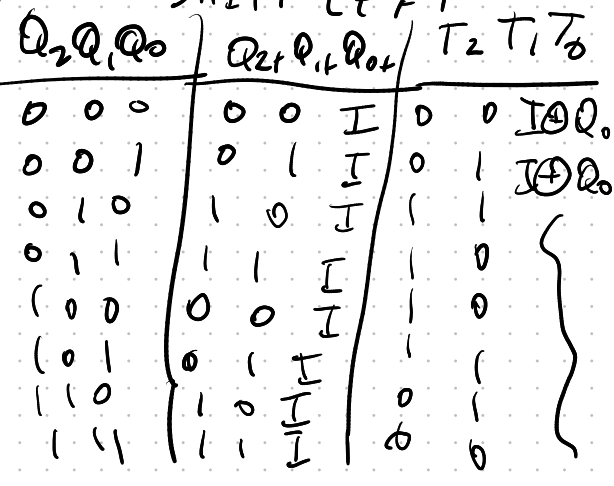
\includegraphics[width=0.5\linewidth]{ex1}
		\end{center}
	
		For the T2 and T1, it is self explanatory. For T0, we need the XOR because again we are using T ffs not D ffs. It makes sense, just trust me. 
		
		Now for the T2 and T1, we need an equation so use 2 k maps to get:
		\begin{align*}
			T_1 = Q_1 \oplus Q_2 \\
			T_2 = Q_2 \oplus Q_1 \\
			T_0 = I\oplus Q_0
		\end{align*}
	
		YAY!! Now we just need 1 more ops. 
		
		\textbf{Count Down: } This is the same process as the shift left. We just need to create the state table, and then find the values for T2T1T0 using K maps: 
		\begin{align*}
			T_0 = 1\\
			T_1 = Q_0 '\\
			T_2 = Q_1 ' Q_0 '
		\end{align*}
	
		Now we are done. We know how to do each of the 3 operations, we just need to \emph{choose} between them. Since we see \textbf{choose}, we know MUX.
		
		We can ignore the last input of our 4x1 muxs since we do not need it. 
		
		\begin{center}
		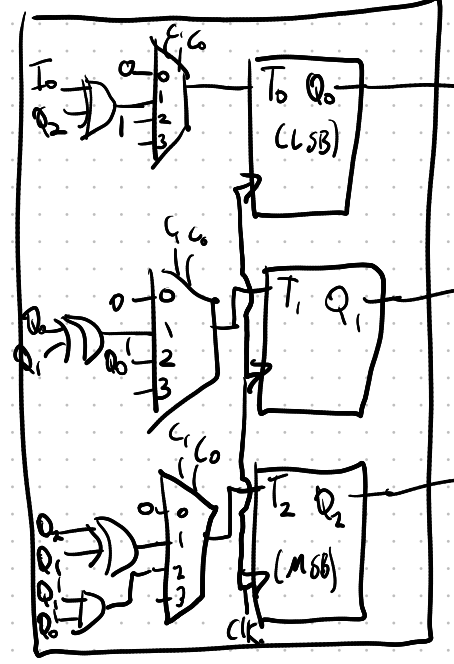
\includegraphics[width=0.5\linewidth]{ex2}
		\end{center}
		
		Most cases are not this bad since we use D flip flops. 
		
		For example, for the left shift using a D, we just put D2 as D1, and D1 as D0, and then D0 as I. SIMPLE!!
		\end{mdframed}
		
		\subsection{Memory}
		If we have $k$ address lines in a memory chip and $n$ data output lines, it means we can store $2^k$ $n$ bit words in that memory chip.
		
		
		\section{Chapter 3}
		\subsection{2s Compliment in Binary}
		To get the 2s compliment of a number in binary, we flip EACH bit (so 1 becomes 0, 0 becomes 1) and then we add 1 to that number. 
		
		Note that when we are using signed numbers where 0 is + and 1 is -, then the 2s compliment of a positive number is itself.  
		
		\subsection{Overflow}
		With signed numbers, overflow occurs when the carry into the sign bit and carry out of the sign bit are different. So:
		\begin{align*}
			OVERFLOW = C_{sign-in} \oplus C_{sign-out}
		\end{align*}
		
		\begin{mdframed}[]
			\textbf{Ex. }
			\begin{center}
			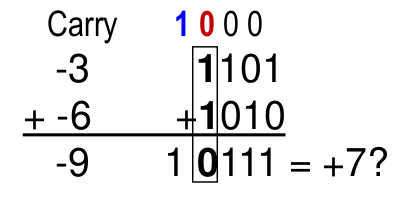
\includegraphics[width=0.3\linewidth]{ex3}
			\end{center}
			Here overflow occurs since the bit into carry 0 is not the same as the bit out of carry 1. 
		
		\end{mdframed}
		
		\subsection{IEEE Floating Point}
		This is a standerdized way of representing floating bit numbers. 
		
		We have 3 parts to the 32 bit number to represent a binary number $n$. 
		\begin{enumerate}[]
			\item Sign (1 bit)
			\item Exponent (8 bits) - 127 + The exponent the fractional part needs to be raised to to get $n$ 
			\item Mantissa (23 bits) - The fractional part of the normalized number $n$
		\end{enumerate}
	
		\begin{mdframed}[]
		\textbf{Ex. Express $(36.5625)_{10}$ as a 32 bit FP number using the IEEE standard.}
		
		The value in binary is $100100.1001$ and normalized is $1.001001001 \times 2^5$.
		
		\begin{enumerate}[noitemsep]
			\item Sign: 0
			\item Exponent: 5+127 = 131 = 10000100 
			\item Mantissa: 00100100100000000000000
		\end{enumerate}
		
		So the 32 bit number is: 0 10000100 00100100100000000000000 (without the spaces ofc)
		\end{mdframed}
		
		\section{Chapter 4}
		
		An operation executed in \textit{one} clock cycle is called a \textbf{micro operation}.
		
		\subsection{Arithmetic Operations}
		These are things such as adding, subtracting, and really anything that uses an adder block.
		
		\subsection{Logic Operations}
		These are things that are not arithmetic but are still done such as AND, OR, SHIFTS, etc.
		
		A circular shift will shift everything left or right and the spare bit will be taken from the other side.
		
		A logical shift will shift everything left or right and the spare bit will be always a 0.
		
		An arithmetic shift will shift everything left or right and the spare bit if right will be the same as the original MSB, and if left will be 0.
		
		Right Arithmetic shift is division, and Left Arithmetic shift is multiplication.
		
		
		
	
	
	
	
\end{document}